\section{Artificial Neural Networks}
% Artificial Neural Networks (ANNs) represent one of the most dynamic research fields in Machine Learning, forming the backbone of deep learning
% —a subset of machine learning that has revolutionized the handling of vast and complex datasets.
% Their architectural foundation resembles the one of the human brain, which ANNs attempt to mimic. In other words, similar to the
% human brain, ANNs consist of layers of interconnected nodes, otherwise known as "neurons", designed to perform specific computational tasks
% ~\cite{dongare_intro_ANN_2012}.

% Several fields have made great progress by utilizing this architecture—namely, image and speech recognition,
% natural language processing, and decision-making under uncertainty have all benefited massively from the application of Neural Networks.
% These immense capabilities of ANNs transfer admirably to a variety of everyday needs, ranging from healthcare diagnostics to autonomous
% vehicles and financial modeling, showcasing noteworthy robustness and versatility\cite{wu_feng_ANN_development_2018}. However, when regarding
% the ANNs described in this research study under the scope of the previously proposed taxonomy (see \cref{fig:ml_taxonomy}), we will focus on
% online learning ANNs that apply task-oriented supervised learning for classification purposes.

Artificial Neural Networks (ANNs) are a pivotal research area in Machine Learning, forming the backbone of deep learning, which has transformed handling
vast and complex datasets. ANNs mimic the human brain's architecture, consisting of layers of interconnected neurons designed for specific computational
tasks~\cite{dongare_intro_ANN_2012}. ANNs have significantly advanced fields such as image and speech recognition, natural language processing, and
decision-making under uncertainty. Their versatility extends to various applications, including healthcare diagnostics, autonomous vehicles, and financial
modeling, demonstrating robustness and adaptability\cite{wu_feng_ANN_development_2018}. This study focuses on online learning ANNs applying supervised learning
for classification.

%%%%%%%%%%%%%%%%%%%%%%%%%%%%%%%%%%%%%%%%%%%%%%%%%%%%%%%%%%%%%%%%%%%%%%%%%%%%%%%%%%%%%%%%%%%%%%%%%%%%%%%%%%%%%%%%%%%%%%%%%%%%%%%%%%%%%%%%%%%%%%%%%%%%%%%%%%%%%%
\subsection{Perceptron and Activation Functions}
\subsubsection{Rosenblatt and Multi-Layer Perceptrons}

Perceptrons, regarded as one of the earliest and simplest forms of artificial neurons, were initially introduced by Frank Rosenblatt in 1958
~\cite{rosenblattPerceptronProbabilisticModel1958}. Perceptrons functionality is closely related to classification tasks and can be
divided into two categories; Rosenblatt Perceptrons and Multi-Layer Perceptrons (MLP).

The first definition of perceptrons resembles a single-layer neural network with $m$ input sources and one sole output neuron,
where stimuli can be classified into two classes, using a linear decision boundary based on the Heaviside function. This single-layer structure,
restricts Rosenblatt perceptron flexibility, limiting its functionality to linearly separable problems and binary classification tasks. To
demonstrate the functionality of this kind of perceptron, a more strict mathematical description seems necessary\cite{zhangArtificialNeuralNetwork2018}:
\begin{equation}
    % \[
    \begin{cases}
        v = \sum_{i=1}^{m} w_i x_i + b, \\
        y = \phi(v)
    \end{cases}
    % \]
    \label{eq:perceptron}
\end{equation}

Expanding on the definition provided by \cref{eq:perceptron}, Consider $x_i$ (for $i = 1, \ldots, m$) as
the set of input signals delivered to a perceptron. In this model, each $w_i$ represents the synaptic weight associated with the perceptron for
the corresponding input $x_i$. The term $b$ is known as the externally set bias. The term $v$ is referred to as the \emph{induced local field}
or simply the linear combiner of inputs and weights. The function $\phi$, which is an activation function or a step function, processes this induced
local field to produce the output $y$ (see \cref{fig:ros_perceptron}) of the perceptron. This perceptron model essentially consists of a linear
combiner capped by a step function, which decisively determines the output based on the calculated local field $v$.

% \cite{zhangArtificialNeuralNetwork2018} -> rosenblatt_perceptron.jpg
\begin{figure}[!ht]
    \centering
    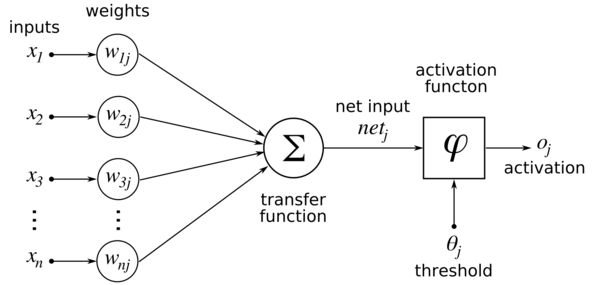
\includegraphics[width=.8\textwidth]{./figures/ann/rosenblatt.png}
    \caption{Simple representation of Rosenblatt’s perceptron.}
    \label{fig:ros_perceptron}
\end{figure}

The activation function of Rosenblatt' perceptron, also referred to as the Heaviside step function, is a straightforward threshold function summarized by \cref{eq:heaviside_step}.
The binary output of the function allows us to determine whether an input sample belongs to one out of two classes limiting strictly in binary classification problems
~\cite{popescuMultilayerPerceptronNeural2009}. For this reason, more adaptable activation functions were introduced for various use cases which will be outlined later:

\begin{equation}
    \phi(v) =
    \begin{cases}
        1 & \text{if } v > 0,    \\
        0 & \text{if } v \leq 0.
    \end{cases}
    \label{eq:heaviside_step}
\end{equation}

% Despite the foundational impact of Rosenblatt's perceptrons in the field of neural networks, the limitation encountered in non-linear
% problems created a gap that needed to be filled by a more sophisticated approach. This need led subsequently to the research and development
% of Multi-Layer Perceptron (MLP) Models, similar to the ones utilized today in neural network applications, providing a solution to the famous XOR problem
% initially stated by Marvin Minsky and Seymour Papert in their book\cite{minskyPerceptronsReissue19882017}. Essentially, the incorporation of
% multiple layers of neurons, including hidden ones, opened the gate for learning intricate patterns within the data, enhancing the learning
% capabilities and potential of the systems with non-linear transformations.

% This fundamental advancement in the field enhanced the network's
% generalization ability by learning hierarchical features from the data and improved its flexibility to adapt to different levels of complexity,
% ranging from simple linear problems to problems with complex decision boundaries that single-layer perceptrons could not handle.

% The architecture of a Multi-Layer Perceptron (MLP) differs substantially from Rosenblatt's approach. To be precise, the architecture of the perceptron
% can be divided into three types of layers.

Despite the foundational impact of Rosenblatt's perceptrons in neural networks, their limitations with non-linear problems created a need for a more sophisticated
approach. This led to the development of Multi-Layer Perceptron (MLP) models, which addressed the famous XOR problem highlighted by Marvin Minsky and Seymour
Papert\cite{minskyPerceptronsReissue19882017}. By incorporating multiple layers of neurons, including hidden ones, MLPs can learn intricate patterns in data,
enhancing their learning capabilities and handling non-linear transformations. This advancement improved the network's generalization ability by learning hierarchical
features and adapting to various levels of complexity, from linear problems to complex decision boundaries that single-layer perceptrons could not manage.

The architecture of a Multi-Layer Perceptron (MLP) differs substantially from Rosenblatt's perceptrons. It consists of three types of layers:

\begin{itemize}
    \item \emph{Input layer:} $n$ source neurons.
    \item \emph{Hidden layers:} one or several hidden layers each containing containing \(h_i\) neurons.
    \item \emph{Output layer:} \(m\) output neurons.
\end{itemize}

Each neuron in the network employs a differentiable non-linear activation function. The most commonly utilized activation function in MLPs
is the sigmoid which is close to linear near the origin while saturating rather quickly when getting away\cite{popescuMultilayerPerceptronNeural2009}. This allows multilayer
perceptrons to model well both strongly and mildly nonlinear relations. Additionally, the structure of this MLP is fully connected, meaning every neuron
in a given layer is connected to all neurons in the subsequent layer (see \cref{fig:multi_perceptron}). Signals in the network flow unidirectionally
from the input layer to the output layer, moving sequentially through each layer from left to right.
\begin{figure}[!ht]
    \centering
    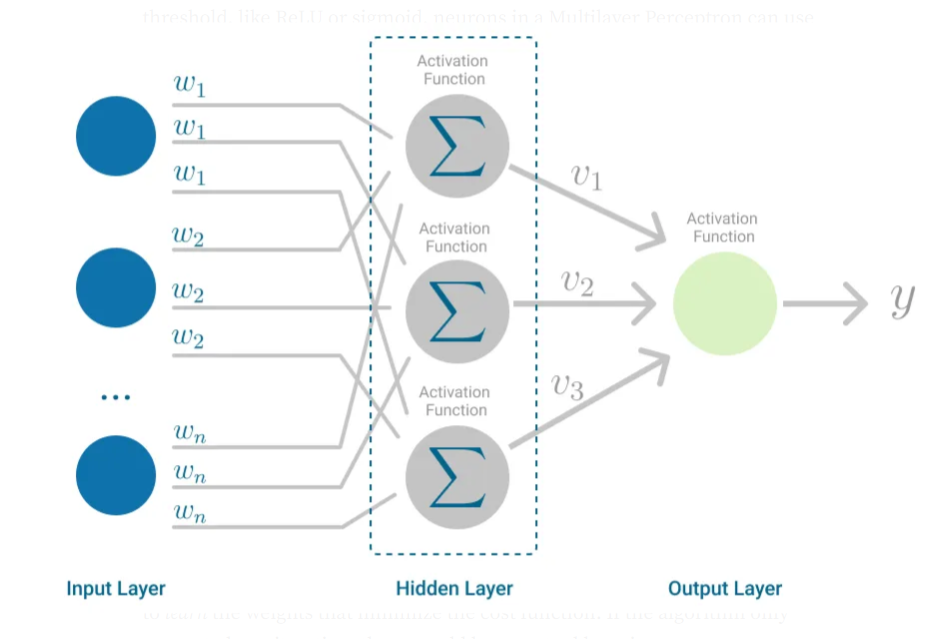
\includegraphics[width=0.75\textwidth, keepaspectratio]{./figures/ann/mlp_2.png}
    \caption{A simple MLP example with $n$ input neurons, one hidden layer with $h_1=3$ neurons and $m=1$ output neuron.}
    \label{fig:multi_perceptron}
\end{figure}




% \cite{zhangArtificialNeuralNetwork2018} -> mlp.png
%%%%%%%%%%%%%%%%%%%%%%%%%%%%%%%%%%%%%%%%%%%%%%%%%%%%%%%%%%%%%%%%%%%%%%%%%%%%%%%
\subsubsection{Evolution of Activation Functions}
The functionality of neural networks is greatly influenced by the choice of activation functions. Initially, Rosenblatt's perceptron used the Heaviside step function,
a basic activation function that activates based on a simple threshold rule.

As neural network theory developed, more flexible activation functions were needed to enable learning in multi-layer architectures and address non-linear classification
problems that single-layer perceptrons could not solve. The sigmoid function emerged as one of the most popular choices for Multi-Layer Perceptrons (MLPs) because of
its continuous and differentiable nature, which is crucial for gradient-based learning algorithms like backpropagation.

Over the years, several other activation functions have been introduced to meet specific requirements of neural network architectures and problems. Common examples
include the hyperbolic tangent (tanh), which is similar to the sigmoid but ranges from -1 to 1, centering the data; the Rectified Linear Unit (ReLU), popular in deep
learning networks due to its efficiency and effectiveness at preventing the vanishing gradient problem\cite{VanishingGradientProblem}; and Softmax, predominantly used
in the output layer of Convolutional Neural Networks (CNNs) to convert logits into a probability distribution over multiple exclusive classes (see \cref{sec:cnn}).

These activation functions have been extensively researched to maximize neural network performance\cite{dubeyActivationFunctionsDeep2022,sharmaACTIVATIONFUNCTIONSNEURAL2020}.
\Cref{table:activation_functions}\footnote{The indexed $v_i$ in Softmax's equation in the table symbolizes the reference to class $i$.}
presents a summary of commonly used activation functions.

\begin{table}[h!]
    \centering
    \begin{tabular}{M{0.15\textwidth} M{0.3\textwidth} M{0.15\textwidth} M{0.3\textwidth}}
        \toprule
        \rowcolor{lightgray}
        \textbf{Function}            & \textbf{Equation}                                                                     & \textbf{Use}              & \textbf{Graph}                                                                      \\
        \midrule
        Heaviside Step               & $\phi(v) = \begin{cases} 1 & \text{if } v > 0 \\ 0 & \text{if } v \leq 0 \end{cases}$ & Binary Classification     & 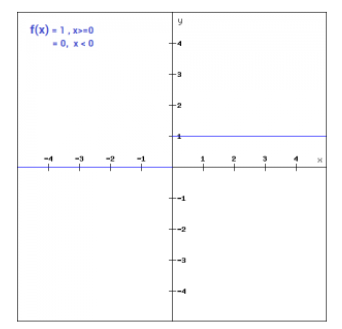
\includegraphics[width=\linewidth, height=25mm]{figures/ann/step_function.png}      \\
        \addlinespace[5pt]
        Sigmoid                      & $\phi(v) = \frac{1}{1 + e^{-v}}$                                                      & Probabilities             & 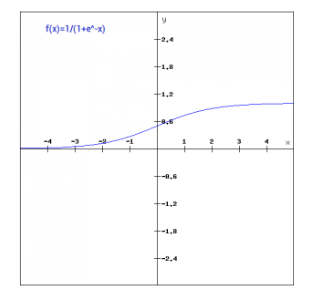
\includegraphics[width=\linewidth, height=25mm]{figures/ann/sigmoid_function.png}   \\
        \addlinespace[10pt]
        Hyperbolic Tangent (tanh)    & $\phi(v) = \frac{e^v - e^{-v}}{e^v + e^{-v}}$                                         & Centered Data             & 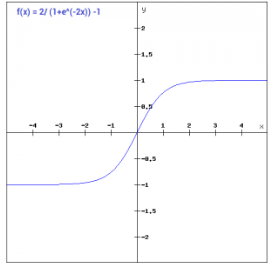
\includegraphics[width=.91\linewidth, height=25mm]{figures/ann/tanh_function.png}   \\
        \addlinespace[10pt]
        Rectified Linear Unit (ReLU) & $\phi(v) = \begin{cases} v & \text{if } v > 0 \\ 0 & \text{if } v \leq 0 \end{cases}$ & Sparse Activation         & 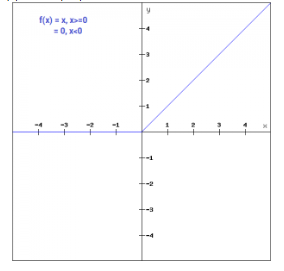
\includegraphics[width=\linewidth, height=25mm]{figures/ann/relu_function.png}      \\
        \addlinespace[10pt]
        Softmax                      & $\phi(v_i) = \frac{e^{v_i}}{\sum_{k} e^{v_k}}$                                        & Multiclass Classification & 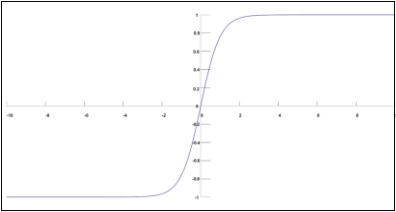
\includegraphics[width=.9\linewidth, height=25mm]{figures/ann/softmax_function.png} \\
        \bottomrule
    \end{tabular}
    \caption{Commonly used activation functions in neural networks\cite{sharmaACTIVATIONFUNCTIONSNEURAL2020}
    }
    \label{table:activation_functions}
\end{table}

These developments have significantly shaped the design and implementation of modern neural networks. The shift from simple threshold functions to complex
non-linear functions has enabled neural networks to model intricate patterns in data, improving their ability to generalize from training data to unseen situations.
This transition marks a pivotal evolution from early perceptrons to the sophisticated networks at the forefront of artificial intelligence research and applications today.



% The functionality of neural networks is greatly influenced by the choice of activation functions. Initially, as with Rosenblatt's perceptron, the $Heaviside$
% step function was the primary activation function used. This simple function determined whether to activate or not based on a simple threshold
% rule.

% As neural network theory developed, the need for more flexible activation functions became apparent, particularly to enable learning in
% multi-layer architectures and to address non-linear classification problems that single-layer perceptrons could not solve. The $sigmoid$ function emerged as one
% of the most popular choices for MLPs because of its continuous and differentiable nature, which is crucial for gradient-based learning algorithms like backpropagation.

% Several other activation functions were introduced in subsequent years depending on the specific requirements of the neural network architecture and the problem at
% hand. Some common examples include the hyperbolic tangent (tanh), which is similar to the sigmoid but ranges from -1 to 1, the Rectified Linear Unit (ReLU),
% which is particularly popular in deep learning networks due to its efficiency and effectiveness at preventing the vanishing gradient problem\cite{VanishingGradientProblem}
% and Softmax, that is predominantly used in the output layer of CNNs (see \cref{sec:cnn}), to convert the logits output into a probability distribution over multiple exclusive
% classes.

% All of the activations
% functions discussed have been thoroughly researched by multiple sources\cite{dubeyActivationFunctionsDeep2022,sharmaACTIVATIONFUNCTIONSNEURAL2020} to examine their
% field of excellence in order to maximize neural network performance. \Cref{table:activation_functions} presents a brief summary.


% \begin{table}[h!]
%     \centering
%     \begin{tabular}{M{0.15\textwidth} M{0.3\textwidth} M{0.15\textwidth} M{0.3\textwidth}}
%         \toprule
%         \rowcolor{lightgray}
%         \textbf{Function}            & \textbf{Equation}                                                                     & \textbf{Use}              & \textbf{Graph}                                                                      \\
%         \midrule
%         Heaviside Step               & $\phi(v) = \begin{cases} 1 & \text{if } v > 0 \\ 0 & \text{if } v \leq 0 \end{cases}$ & Binary Classification     & 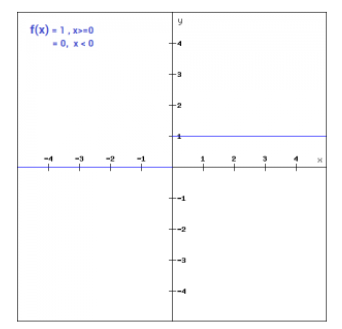
\includegraphics[width=\linewidth, height=25mm]{figures/ann/step_function.png}      \\
%         \addlinespace[5pt]
%         Sigmoid                      & $\phi(v) = \frac{1}{1 + e^{-v}}$                                                      & Probabilities             & 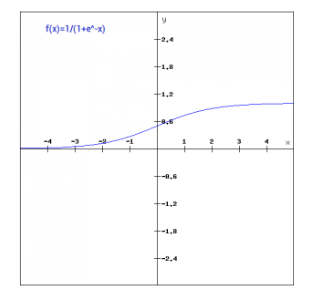
\includegraphics[width=\linewidth, height=25mm]{figures/ann/sigmoid_function.png}   \\
%         \addlinespace[10pt]
%         Hyperbolic Tangent (tanh)    & $\phi(v) = \frac{e^v - e^{-v}}{e^v + e^{-v}}$                                         & Centered Data             & 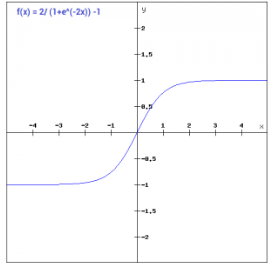
\includegraphics[width=.91\linewidth, height=25mm]{figures/ann/tanh_function.png}   \\
%         \addlinespace[10pt]
%         Rectified Linear Unit (ReLU) & $\phi(v) = \begin{cases} v & \text{if } v > 0 \\ 0 & \text{if } v \leq 0 \end{cases}$ & Sparse Activation         & 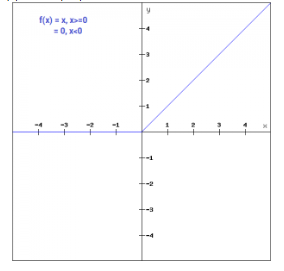
\includegraphics[width=\linewidth, height=25mm]{figures/ann/relu_function.png}      \\
%         \addlinespace[10pt]
%         Softmax                      & $\phi(v_i) = \frac{e^{v_i}}{\sum_{k} e^{v_k}}$                                        & Multiclass Classification & 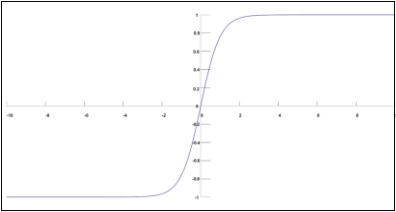
\includegraphics[width=.9\linewidth, height=25mm]{figures/ann/softmax_function.png} \\
%         \bottomrule
%     \end{tabular}
%     \caption{Commonly used activation functions in neural networks\cite{sharmaACTIVATIONFUNCTIONSNEURAL2020}
%         \emph{Comment:} The indexed $v_i$ in Softmax symbolizes the reference to class $i$.}
%     \label{table:activation_functions}
% \end{table}

% These developments have significantly shaped the design and implementation of modern neural networks. The advancement from simple threshold functions
% to complex non-linear functions has enabled neural networks to model intricate patterns in data, improving their ability to generalize from training
% data to unseen situations. This transition marks a pivotal evolution from early perceptrons to the sophisticated networks that are at the forefront
% of artificial intelligence research and applications today.

%%%%%%%%%%%%%%%%%%%%%%%%%%%%%%%%%%%%%%%%%%%%%%%%%%%%%%%%%%%%%%%%%%%%%%%%%%%%%%%%%%%%%%%%%%%%%%%%%%%%%%%%%%%%%%%%%%%%%%%%%%%%%%%%%%%%%%%%%%%%%%%%%%%%%%%%%%%%%%
\subsection{Network Architectures}
The research in the domain of neural networks always strives for optimization, and to be precise, maximization of performance and generalization\cite{ransisiNeuralNetworkTypes2021}.
Hence, in an effort to expand the limits of what can be achieved with Neural Networks, several diverse architectures have been proposed, tailored
for specific data and fields. That way performance is improved by addressing the specific needs of a given problem. While the types of architectures
developed to this day are countless, this analysis will be restricted to a brief overview of two major categories and afterward, there will be a shift in focus
toward the architecture most valuable for this research.

\begin{figure}[h!]
    \centering
    \begin{subfigure}[t]{0.49\textwidth}
        \centering
        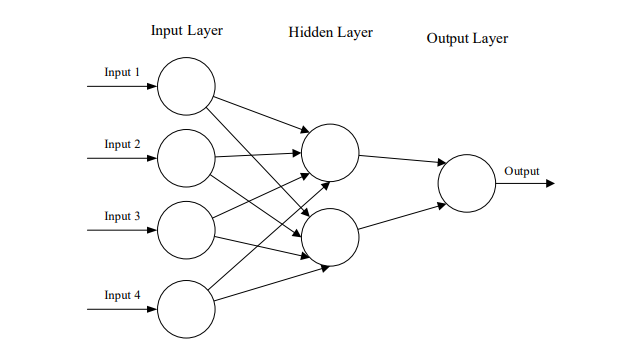
\includegraphics[width=1.1\textwidth,height=.6\textwidth]{figures/ann/ffnn.png}
        \caption{FFNN with one hidden layer\cite{osheaIntroductionConvolutionalNeural2015}.}
        \label{fig:ffnn}
    \end{subfigure}\hfill
    \begin{subfigure}[t]{0.49\textwidth}
        \centering
        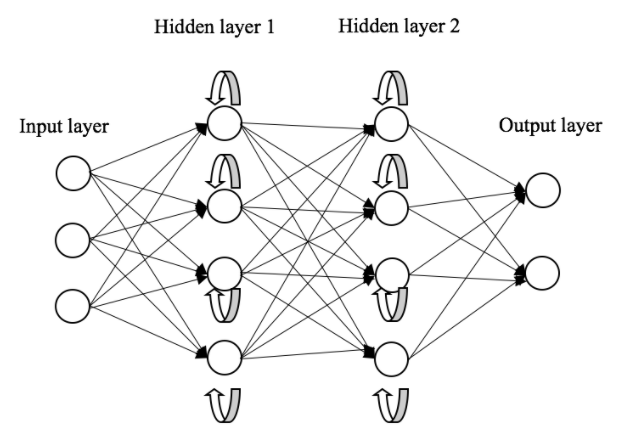
\includegraphics[width=\textwidth]{figures/ann/rnn1.png}
        \caption{General structure of RNNs\cite{communityUnderstandingMechanismTypes2020}.}
        \label{fig:rnn}
    \end{subfigure}
    \caption{A side by side illustration of FFNN and RNN architectures.}
    \label{fig:ffnn_rnn}
\end{figure}

First and foremost, there are Feed-Forward Neural Networks (FFNN)\cite{leshnoMultilayerFeedforwardNetworks1993} which represents the simplest form of
neural network, designed on the tracks of MLPs' logic discussed previously (see \cref{fig:ffnn}). In this type of networks, neurons are organized
in layers with each neuron being connected to all neurons of subsequent layers. The network's flow is unidirectional from the input layer through hidden
layers to the output layer. Common use examples contain image and speech recognition, due to their simplicity and effectiveness.

Moving forward, another crucial type of neural network architecture is Recurrent Neural Networks (RNNs)\cite{communityUnderstandingMechanismTypes2020}.
Recurrent Neural Networks are designed to handle sequential data\cite{ghiassiDynamicArtificialNeural2005}. Differing from traditional neural networks, RNNs process inputs
using a loop mechanism that allows information from previous steps to influence current and future operations (see \cref{fig:rnn}). This architecture
~\cite{osheaIntroductionConvolutionalNeural2015} makes RNNs ideal for applications such as language modeling and text generation, where the sequence and context
of information are critical. They are particularly effective in tasks like speech recognition, music generation, and other forms of sequential pattern recognition.

%%%%%%%%%%%%%%%%%%%%%%%%%%%%%%%%%%%%%%%%%%%%%%%%%%%%%%%%%%%%%%%%%%%%%%%%%%%%%%%
\subsubsection{Convolutional Neural Networks (CNNs)}
\label{sec:cnn}
% Building on the foundational principles laid out by Feed-Forward Neural Networks, the exploration into network architectures takes a sophisticated turn
% with Convolutional Neural Networks (CNNs)\cite{guRecentAdvancesConvolutional2018}, arguably one of the most significant achievements of Deep Learning.
% CNNs have known great applicability in several fields including image and video recognition, recommendation systems, image classification, image
% segmentation natural language processing, and computer vision. The name of CNNs stems from the \emph{convolution}-an operation described in calculus,
% as a mathematical operation that combines two functions to produce a third, that expresses how the shape of one is modified by the other.
% This inherent property of convolutional layers provides CNNs with translation-invariance, enabling them to detect and extract patterns and
% features from data regardless of changes in position, orientation, scale, or translation.

Building on the foundational principles of Feed-Forward Neural Networks, the exploration into network architectures takes a sophisticated turn with Convolutional
Neural Networks (CNNs)\cite{guRecentAdvancesConvolutional2018}, a significant achievement in Deep Learning. CNNs have broad applicability in fields such as image
and video recognition, recommendation systems, image classification, image segmentation, natural language processing, and computer vision. The name of CNNs stems
from the \emph{convolution}-an mathematical operation described in calculus that combines two functions to produce a third, that expresses how the shape of one
is modified by the other. This inherent property of convolutional layers provides CNNs with translation-invariance, enabling them to detect and extract patterns and features
from data regardless of position, orientation, scale, or translation.

\begin{figure}[!ht]
    \centering
    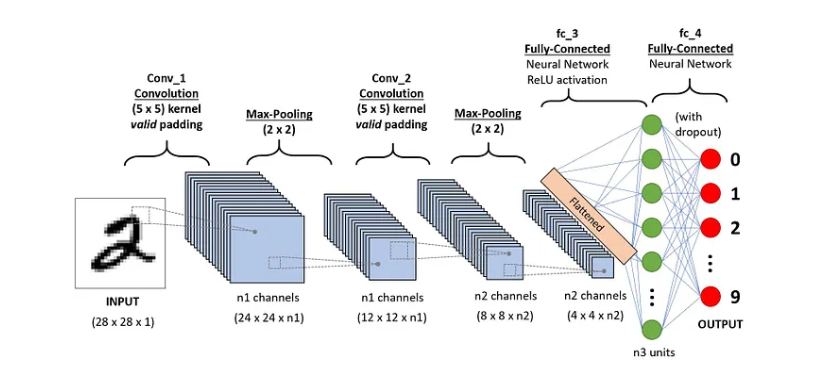
\includegraphics[width=\textwidth]{figures/ann/cnn1.png}
    \caption{A CNN sequence to classify handwritten digits\cite{sahaComprehensiveGuideConvolutional2022}}
    \label{fig:cnn}
\end{figure}

To further elucidate the methodology of a CNN, we will observe the example of \cref{fig:cnn} depicting a single input from the MNIST dataset\footnote{Dataset of handwritten digits}
while being processed. The format in which the system perceives the input is a pixel representation of the image. After the input is received the sample
undergoes a series of critical operations that eventually lead to the system's output.


The \emph{convolution layer} performs a sliding window function to the matrix of pixels representing the digit's image, commonly known as kernel or filter.
Several filters of equal size are applied, and each filter is used to recognize a specific pattern from the image, generating multiple feature maps.
Observing \cref{fig:cnn}, a $4(height)x4(breadth)$ kernel is utilized, sliding over the input image, calculating the convolution result at each point
and populating the feature map.

\begin{figure}[!ht]
    \centering
    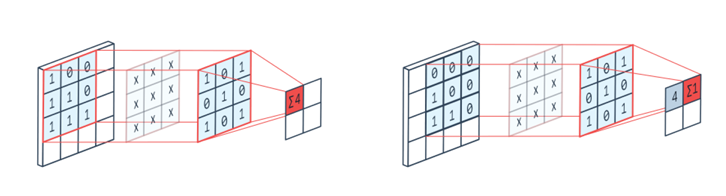
\includegraphics[width=1\textwidth,keepaspectratio]{figures/ann/convolutional_layer.png}
    \caption{A convolution of a $4\times4$ image with a $3\times3$ kernel highlighting the sliding window operation\cite{petrakosemmanouelReconfigurableLogicFPGA2023}}
    \label{fig:kernel}
\end{figure}

After each convolution operation, a ReLU (see \cref{table:activation_functions}) activation function is applied to
deduce non-linear relationships between the features in the image, hence improving the network's capability for
capturing complex patterns.

Following the convolution and activation steps, the \emph{pooling (or subsampling) layer} reduces the spatial dimensions of the feature maps. This step is crucial as it
decreases computational requirements and the number of parameters, helping prevent overfitting. Max pooling, which selects the maximum value from each patch of the
feature map, is the most frequently used method (\cref{fig:max_pooling}). Another common method is average pooling, which calculates the average value of each patch (\cref{fig:avg_pooling}).
The final pooling layer converts the feature map into a flattened, one-dimensional array, preparing it for input into the fully connected layer.

\begin{figure}[!ht]
    \centering
    \begin{subfigure}[b]{0.49\textwidth}
        \centering
        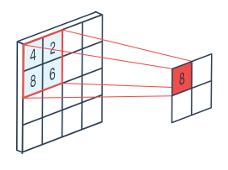
\includegraphics[width=.6\textwidth]{figures/ann/max_pooling.png}
        \caption{Max pooling}
        \label{fig:max_pooling}
    \end{subfigure}
    \hfill
    \begin{subfigure}[b]{0.49\textwidth}
        \centering
        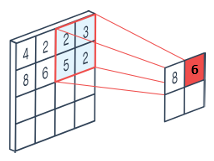
\includegraphics[width=.58\textwidth]{figures/ann/avg_pooling.png}
        \caption{Average pooling}
        \label{fig:avg_pooling}
    \end{subfigure}
    \caption{Demosntration of max and avergae pooling operations.}
    \label{fig:max_and_avg_pooling}
\end{figure}


The \emph{fully connected layers} represent the last layer of a CNN and their inputs correspond to the flattened one-dimensional matrix generated by the last pooling layer.
ReLU activations functions are applied to them for non-linearity again (as shown in \cref{fig:cnn}).
Finally, a softmax prediction layer is used to generate probability values for each of the possible output labels, and the final label predicted is the one with
the highest probability score.
%%%%%%%%%%%%%%%%%%%%%%%%%%%%%%%%%%%%%%%%%%%%%%%%%%%%%%%%%%%%%%%%%%%%%%%%%%%%%%%
%%%%%%%%%%%%%%%%%%%%%%%%%%%%%%%%%%%%%%%%%%%%%%%%%%%%%%%%%%%%%%%%%%%%%%%%%%%%%%%%%%%%%%%%%%%%%%%%%%%%%%%%%%%%%%%%%%%%%%%%%%%%%%%%%%%%%%%%%%%%%%%%%%%%%%%%%%%%%%
\subsection{Learning in Neural Networks}
Having established the principal components and architecture of ANNs, we proceed with a brief demonstration of their learning method.
Learning in neural networks, achieved by training\footnote{Training is also called fitting in ML terminology}, involves the adjustment of the network’s
internal parameters to minimize the discrepancy between the actual output and the target output. This process is crucial for developing models that
can perform well on unseen data. Yet, In order to successfully grasp the reasoning behind the training process, it is crucial to decompose the procedure into
smaller, comprehensive, sub-processes.\cite{martyNeuralNetworksLearning2023}. In essence, this analysis partitions the training process into six parts as follows;

\begin{enumerate}
    \item \emph{Initialization:} The initialization of weights is a critical first step in the training of neural networks. Proper initialization sets the stage for
          an efficient and effective learning process, influencing how quickly a network converges to a solution, if at all. Initially, weights can be set randomly,
          but more sophisticated methods such as He initialization or Xavier initialization are commonly used to improve the convergence properties of deep networks\cite{goodfellowDeepLearning2016}.
          These methods adjust the scale of the weights according to the number of input and output neurons, promoting an even
          distribution of activations across layers during the initial phases of training\cite{narkhedeReviewWeightInitialization2022}.

    \item \emph{Forward Propagation:} This step involves computing the output of a neural network, starting by feeding the input data and calculating the weighted
          sum of each neuron's inputs. The activation or non-activation of the neuron is determined by the output of the nonlinear activation function (see \cref{table:activation_functions})
          over the calculated sum. The process begins at the input layer and proceeds sequentially through the hidden layers and finally to the output layer, where a
          prediction is made. The specific transformations applied to the neurons' sums depend on the network's architecture (e.g., convolutional, recurrent) and the types
          of layers used\cite{nielsenNeuralNetworksDeep}.

    \item \emph{Loss Computation:} A cost (or loss) function, quantifies the error between the predicted outputs and the actual target values.
          The cost function selection can significantly affect the network's performance and convergence. Common choices include Mean Squared Error (MSE) for regression
          tasks and Cross-Entropy Loss for classification tasks. The cost function provides a performance measure used during backpropagation to adjust the model’s weights.

    \item \emph{Back Propagation:} Backpropagation is the fundamental algorithm for training artificial neural networks. It calculates the gradients of the loss function
          with respect to the weights of the network by applying the chain rule of calculus. These gradients indicate the necessary adjustments to the weights to
          minimize the loss function and improve model accuracy. The process involves propagating the error backward through the network, updating the weights to
          reduce the prediction error for subsequent iterations\cite{cilimkovicNeuralNetworksBack}.

    \item \emph{Gradient Descent:} The gradients calculated during the \textit{back propagation phase} comprise a clear indication of the steepest ascent
          on the loss curve, meaning the direction of the maximizing loss. On the contrary, as the objective is to minimize the loss, it becomes obvious that the
          required update of the network’s parameters needs to be performed moving in the opposite direction of the gradients. By iteratively adjusting the weights
          in this direction, the accuracy of the system increases, while The magnitude of this update is controlled by a learning rate hyperparameter of the
          optimization algorithm. Additional information for this matter will be presented in the following \cref{sec:optimization}.

    \item \emph{Iteration:} Steps $2-5$ are repeated for each batch of training data for multiple epochs\footnote{Epoch is a complete pass over the training dataset} until
          the neural network’s performance on the training data achieves convergence to a solution.

\end{enumerate}

The above process is repeated iteratively until the breaking condition is satisfied. However,
this does not necessarily guarantee generalization. The above statement loops back to a previously reported
issue in machine-learning-overfitting (see \cref{sub2:overfitting}). Therefore, training can include a validation
step where the model is tested on unseen data to adjust hyperparameters and prevent overfitting.

In closing analysis, it should be noted that the neural networks, as demonstrated, accumulate knowledge
by iterative adjusting the network's parameters based on the optimization algorithm applied.
This suggests that a vast number of operations need to be performed at each training step.
In restricted-size models, the above operation may be a manageable load for the computers to handle,
then again this is not the fact, for substantially sized networks, where the computational demands can become
humongous. Hence, training neural networks is typically performed on powerful hardware or specialized hardware
accelerators (GPUs or TPUs) to speed up the process\cite{martyNeuralNetworksLearning2023}.

%%%%%%%%%%%%%%%%%%%%%%%%%%%%%%%%%%%%%%%%%%%%%%%%%%%%%%%%%%%%%%%%%%%%%%%%%%%%%%%%%%%%%%%%%%%%%%%%%%%%%%%%%%%%%%%%%%%%%%%%%%%%%%%%%%%%%%%%%%%%%%%%%%%%%%%%%%%%%%